\documentclass[border=20pt]{standalone}
\usepackage[T1]{fontenc}
\usepackage{lmodern}
\usepackage{tikz}
\usetikzlibrary{positioning,arrows.meta,calc,shapes.geometric,backgrounds}

% Define editorial palette matching the poster
\definecolor{paper}{HTML}{F6F1E7}
\definecolor{card}{HTML}{FAFAF6}
\definecolor{cardTan}{HTML}{F0EBDD}
\definecolor{stroke}{HTML}{E1DBCE}
\definecolor{ink}{HTML}{0E2747}
\definecolor{accent}{HTML}{E8573F}
\definecolor{muted}{HTML}{5B6680}
\definecolor{groundFill}{HTML}{0E2747}

\begin{document}
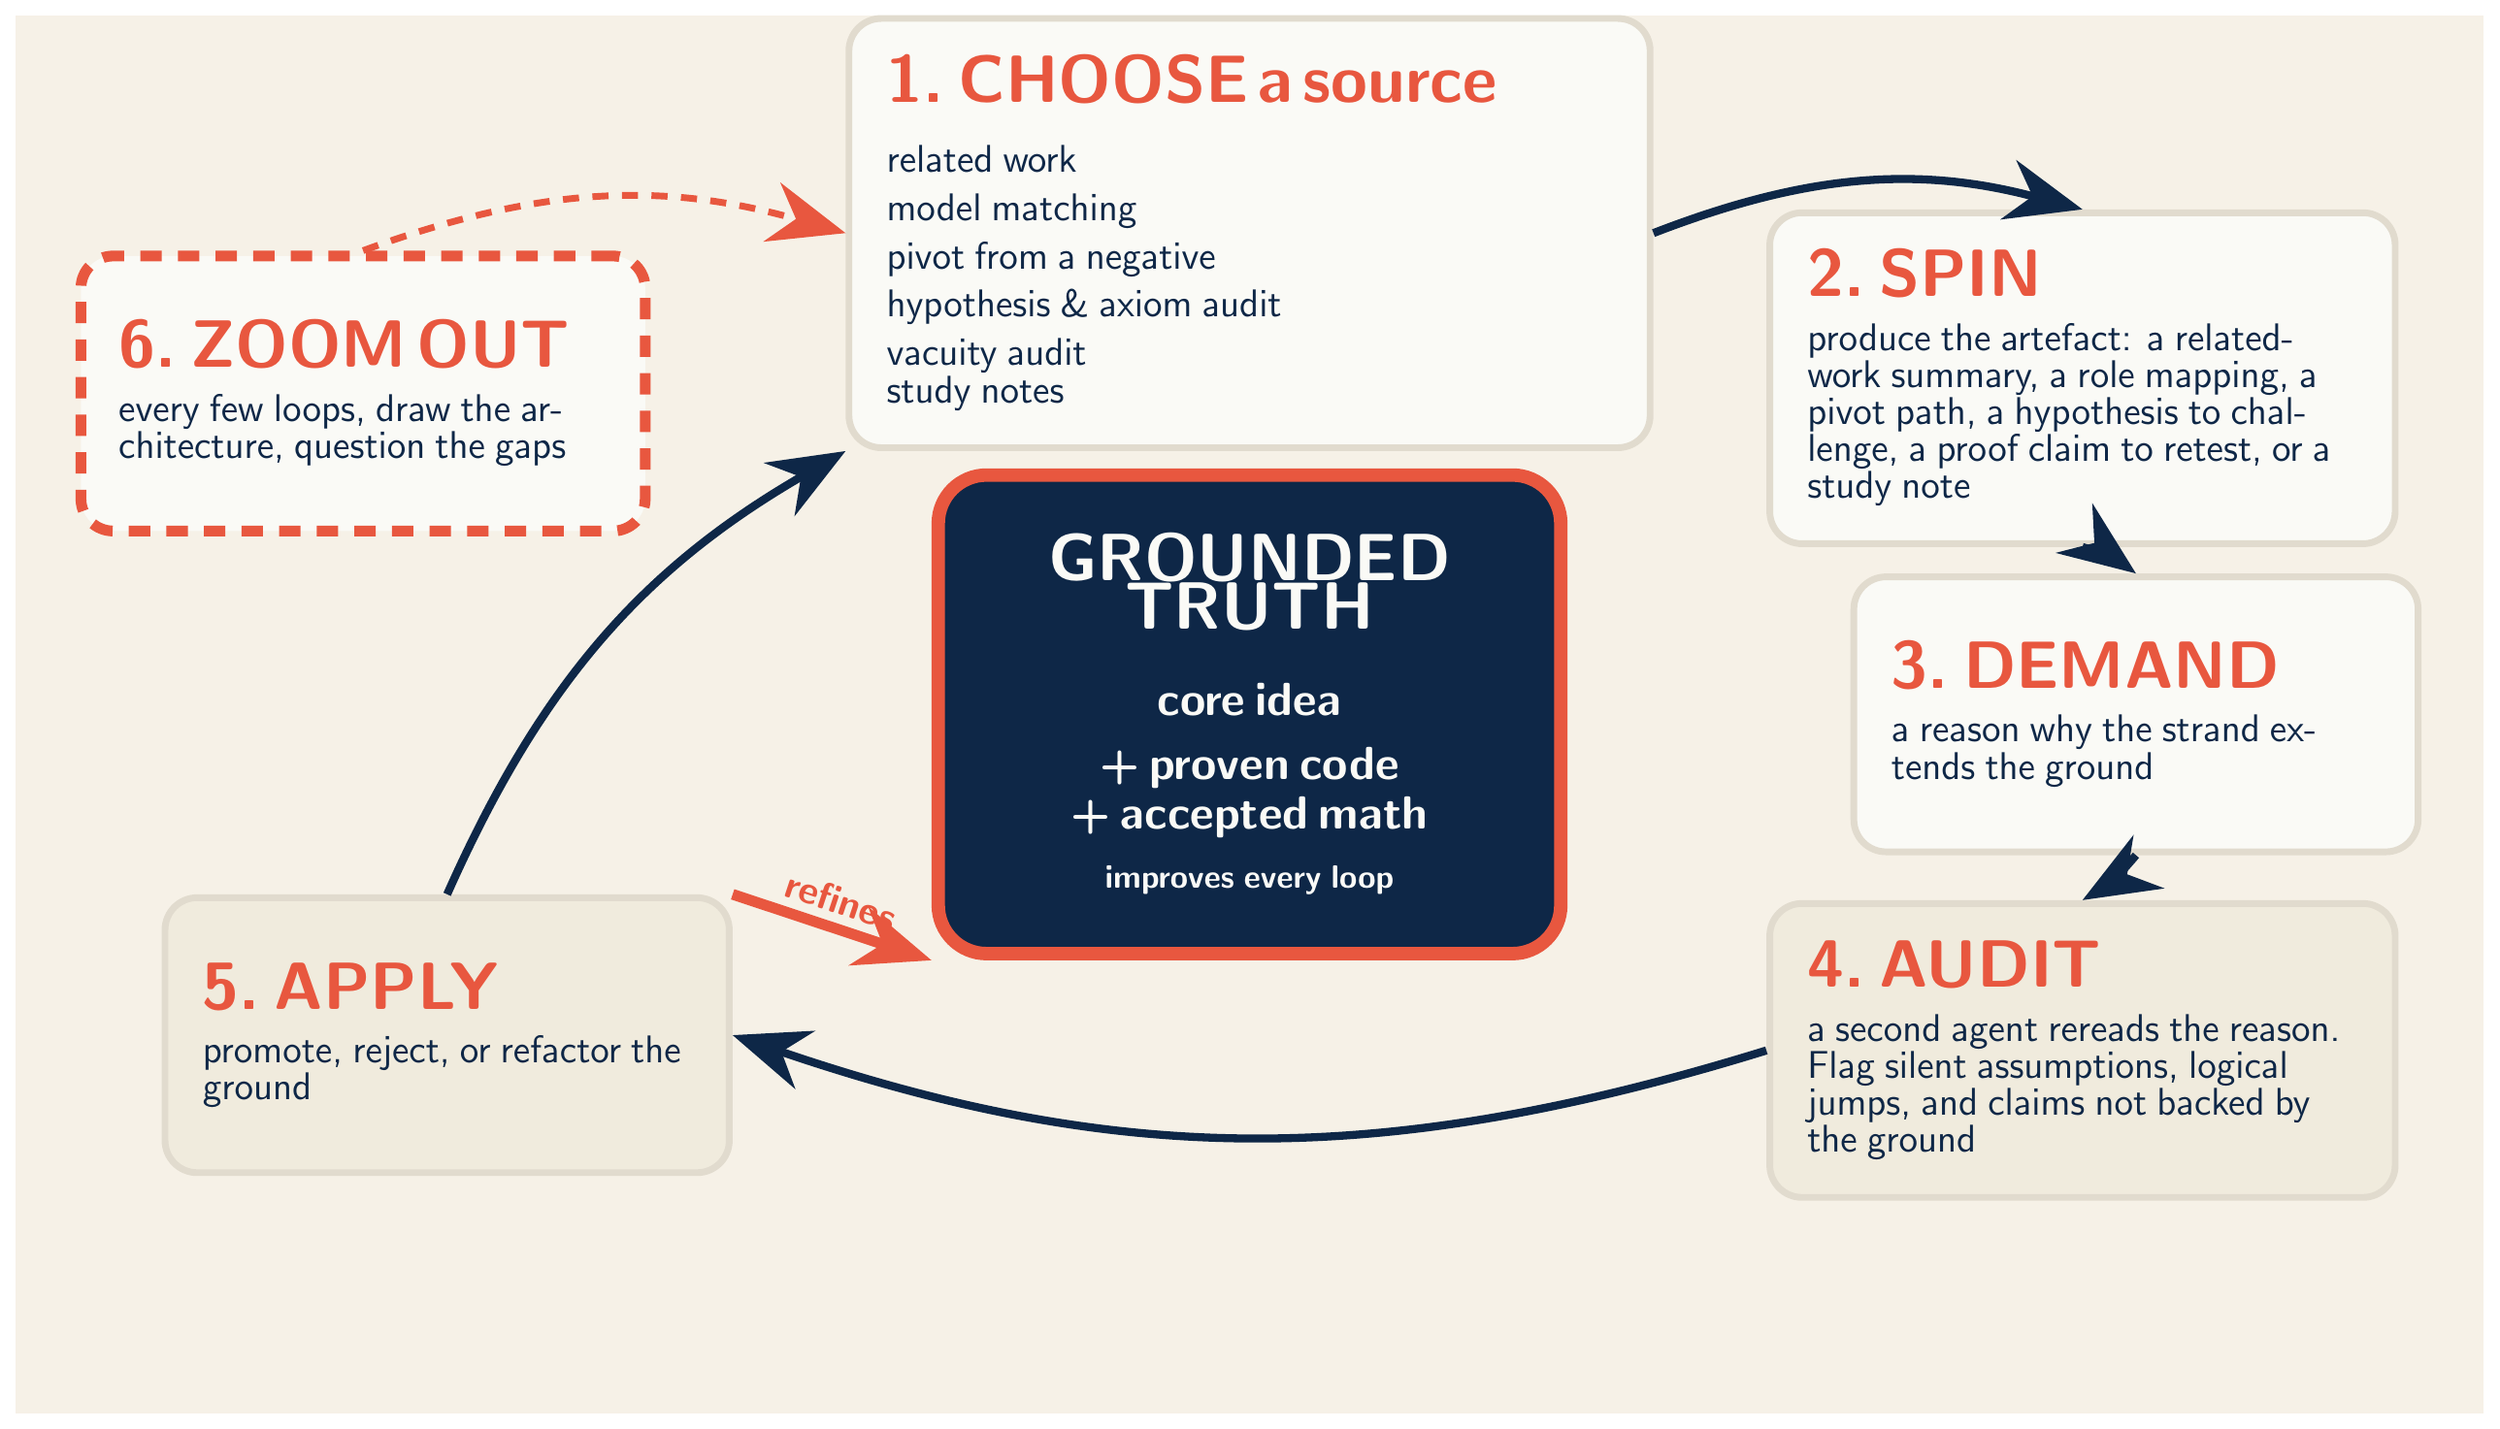
\begin{tikzpicture}[
  font=\sffamily\bfseries,
  background rectangle/.style={fill=paper},
  show background rectangle,
  station/.style={
    rectangle, rounded corners=12pt,
    draw=stroke, line width=2.5pt,
    fill=card,
    inner sep=14pt,
    text width=6.4cm,
    align=left,
    minimum height=3.6cm,
    text=ink
  },
  inwardStation/.style={
    station,
    fill=cardTan
  },
  zoomStation/.style={
    station,
    fill=card,
    draw=accent,
    dash pattern=on 8pt off 6pt,
    line width=4pt
  },
  ground/.style={
    rectangle, rounded corners=18pt,
    draw=accent, line width=5pt,
    fill=groundFill,
    inner sep=22pt,
    text width=6.6cm,
    align=center,
    text=card
  },
  cycleArrow/.style={
    -{Stealth[length=10mm,width=8mm]},
    line width=3pt,
    draw=ink
  },
  refine/.style={
    -{Stealth[length=10mm,width=8mm]},
    line width=4pt,
    draw=accent
  },
  zoomArrow/.style={
    -{Stealth[length=10mm,width=8mm]},
    line width=2.5pt,
    draw=accent,
    dash pattern=on 6pt off 5pt
  }
]

% Text macros for inside nodes
\newcommand{\stationTitle}[1]{{\sffamily\Huge\bfseries\color{accent}#1}}
\newcommand{\stationBody}[1]{{\sffamily\Large\mdseries\color{ink}#1}}
\newcommand{\groundTitle}[1]{{\sffamily\Huge\bfseries\color{card}#1}}
\newcommand{\groundBody}[1]{{\sffamily\LARGE\bfseries\color{card}#1}}

% Force 16:9 bounding box, total figure 32cm x 18cm
\useasboundingbox (-16, -9) rectangle (16, 9);

% Central ground
\node[ground] (G) at (0, 0) {%
  \groundTitle{GROUNDED\\TRUTH}\\[10pt]
  \groundBody{core idea\\[2pt] + proven code\\[2pt] + accepted math}\\[10pt]
  {\sffamily\large\itshape\color{card!90} improves every loop}
};

% 1. CHOOSE (top centre)
\node[station, text width=9.5cm] (s1) at (0, 6.3) {%
  \stationTitle{1. CHOOSE a source}\\[8pt]
  \stationBody{related work\\
  model matching\\
  pivot from a negative\\
  hypothesis \& axiom audit\\
  vacuity audit\\
  study notes}
};

% 2. SPIN (top right)
\node[station, text width=7.2cm] (s2) at (10.9, 4.4) {%
  \stationTitle{2. SPIN}\\[8pt]
  \stationBody{produce the artefact: a related-work summary, a role mapping, a pivot path, a hypothesis to challenge, a proof claim to retest, or a study note}
};

% 3. DEMAND (right)
\node[station] (s3) at (11.6, 0) {%
  \stationTitle{3. DEMAND}\\[8pt]
  \stationBody{a reason why the strand extends the ground}
};

% 4. AUDIT (bottom right)
\node[inwardStation, text width=7.2cm] (s4) at (10.9, -4.4) {%
  \stationTitle{4. AUDIT}\\[8pt]
  \stationBody{a second agent rereads the reason. Flag silent assumptions, logical jumps, and claims not backed by the ground}
};

% 5. APPLY (bottom left)
\node[inwardStation] (s5) at (-10.5, -4.2) {%
  \stationTitle{5. APPLY}\\[8pt]
  \stationBody{promote, reject, or refactor the ground}
};

% 6. ZOOM OUT (left)
\node[zoomStation] (s6) at (-11.6, 4.2) {%
  \stationTitle{6. ZOOM OUT}\\[8pt]
  \stationBody{every few loops, draw the architecture, question the gaps}
};

% Cycle arrows: 1 -> 2 -> 3 -> 4 -> 5 -> back to 1
\draw[cycleArrow] (s1.east) to[bend left=18] (s2.north);
\draw[cycleArrow] (s2.south) to[bend left=10] (s3.north);
\draw[cycleArrow] (s3.south) to[bend left=10] (s4.north);
\draw[cycleArrow] (s4.west) to[bend left=18] (s5.east);
\draw[cycleArrow] (s5.north) to[bend left=18] (s1.south west);

% Periodic zoom-out: 6 cuts back into 1
\draw[zoomArrow] (s6.north) to[bend left=18] (s1.west);

% Refinement: 5 writes into the centre
\draw[refine] (s5.north east) -- (G.south west) node[midway, above, sloped, font=\sffamily\Large\bfseries, text=accent] {refines};

\end{tikzpicture}
\end{document}
